% Gemini theme
% Adapted for: Compile-Time vs. Runtime Trade-offs in Systems Programming
% Authors: Daniel Borgs

\documentclass[final]{beamer}

\usepackage[T1]{fontenc}
\usepackage{lmodern}
\usepackage[size=custom,width=70,height=96,scale=1.0]{beamerposter}
\usetheme{gemini}
\usecolortheme{uchicago}
\usepackage{graphicx}
\usepackage{booktabs}
\usepackage{tikz}
\usepackage{pgfplots}
\usepackage{svg}
\usepackage{minted}
\usepackage{xcolor}
\pgfplotsset{compat=1.17}

\setminted{
	fontsize=\small,
	breaklines=true,
	frame=none,
	xleftmargin=0pt
}

\newlength{\sepwidth}
\newlength{\colwidth}
\setlength{\sepwidth}{0.02\paperwidth}
\setlength{\colwidth}{0.47\paperwidth}

\newcommand{\separatorcolumn}{\begin{column}{\sepwidth}\end{column}}
\renewcommand{\heading}[1]{\vspace{0.5em}\textbf{#1}\vspace{0.3em}\\}

\title{
	Zero-Cost State Management:\\
	Rust Typestate vs. C Runtime Checks
}

\author{Daniel Borgs \and Shiwei Cui \and Taylan Yıldırım}

\institute[shortinst]{Technical University of Applied Sciences W\"urzburg-Schweinfurt}

\footercontent{
	\large
	Professional Skills -- Winter Semester 2025/26
}

\linespread{0.95}
\begin{document}
\addtobeamertemplate{headline}{}
{
	\begin{tikzpicture}[remember picture,overlay]
	\node [anchor=north west, inner sep=3cm] at ([xshift=0.0cm,yshift=-1.8cm]current page.north west)
	{\includesvg[height=3.5cm,inkscapelatex=false]{logos/THWS.svg}};
	\end{tikzpicture}
}

\begin{frame}[t,fragile]
\begin{columns}[t]
\separatorcolumn

\begin{column}{\colwidth}

	\begin{alertblock}{Take-Home Message}
		\large
		\textbf{The Safety-Performance Dilemma}
		
		Programs must ensure operations happen in valid order. A file must be opened before reading. Traditional solutions force a choice:
		\begin{itemize}
			\item \textbf{Safe code}: Check validity at runtime $\rightarrow$ slower execution
			\item \textbf{Fast code}: Skip checks $\rightarrow$ risk of crashes and security holes
		\end{itemize}
		\vspace{0.8cm}

		\textbf{Our Question:} Can we get safety \textit{without} paying the runtime cost?
		\vspace{0.8cm}

		\textbf{Key Finding:} \textbf{Yes.} Rust's type system catches invalid operations during compilation. The resulting program runs as fast as code with no safety checks---while preventing errors that would crash unsafe code.
	\end{alertblock}

	\begin{block}{Problem Statement}
		\large
		\heading{Why This Matters}

		Memory safety bugs dominate security vulnerabilities:
		\begin{itemize}
			\item 70\% of Microsoft's security issues stem from memory safety problems
			\item The Heartbleed bug (2014) exposed millions of servers due to one missing bounds check
			\item The US government now recommends memory-safe languages
		\end{itemize}

		\heading{The Core Tension}

		Systems code (operating systems, databases, embedded devices) requires maximum performance. Safety checks consume CPU cycles. Developers face an uncomfortable choice: \textbf{safe or fast?}

		\heading{State Management}

		Many bugs arise from \textit{state violations}: using an object incorrectly for its current state. Reading from a closed file handle causes undefined behavior---the program might crash, corrupt data, or create a security hole.
	\end{block}
 
	\begin{block}{Background: What Is a State Machine?}
		\large
		\heading{Definition}

		A \textbf{state machine} defines: (1) states an object can be in, (2) valid transitions between states, and (3) operations permitted in each state.

		\begin{figure}
			\centering
			\includesvg[width=0.9\colwidth,inkscapelatex=false]{../paper/svg/state_machine_manual_bottom.svg}
		\end{figure}
	\end{block}

	\begin{block}{The Verification Problem}
		\large
		How do we ensure programs follow state machine rules?

		\begin{table}[]
			\renewcommand{\arraystretch}{1.3}
			\centering
			\begin{tabular}{l|l|l}
				\textbf{Approach} & \textbf{When Checked} & \textbf{Cost} \\
				\hline
				Runtime checks & During execution & CPU cycles, branches \\
				Documentation & Never (honor system) & Zero, but unsafe \\
				Type system & During compilation & \textbf{Zero at runtime} \\
			\end{tabular}
		\end{table}
	\end{block}

\end{column}

\separatorcolumn

\begin{column}{\colwidth}

	\begin{block}{The Typestate Pattern Explained}
		\large
		\heading{Core Idea}

		Instead of one \texttt{FileHandle} type with a state field, create separate types:
		\texttt{FileHandle<Closed>}, \texttt{FileHandle<Open>}, \texttt{FileHandle<Readable>}.

		\heading{How It Prevents Errors}
		
		The \texttt{read()} method is defined \textit{only} for \texttt{FileHandle<Open>}. Attempting to call \texttt{read()} on a \texttt{FileHandle<Closed>} produces a \textbf{compile-time error}---the method does not exist for that type.

		\heading{Why Zero Cost?}

		The state marker (\texttt{<Open>}, \texttt{<Closed>}) exists only for the compiler. It occupies \textbf{zero bytes} in memory and generates \textbf{zero instructions}. After compilation, the type information is erased---only the operations remain.
	\end{block}

	\begin{block}{Results: Assembly Comparison}
		\large
		\heading{Methodology}

		Compiled all three versions at \texttt{-O2} optimization, analyzed generated ARM64 assembly, counted total instructions and conditional branches.

		\begin{figure}
			\centering
			\begin{tabular}{c c}
				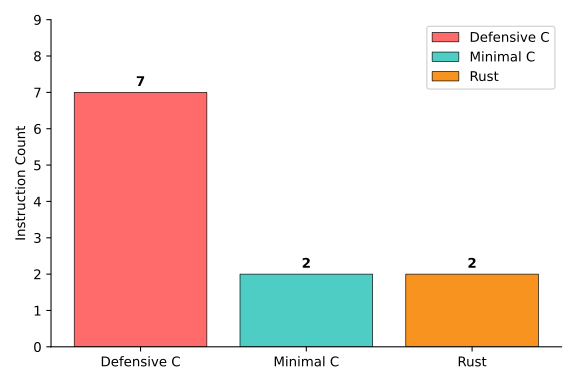
\includegraphics[width=0.48\colwidth]{../paper/figures/instruction_count.pdf} &
				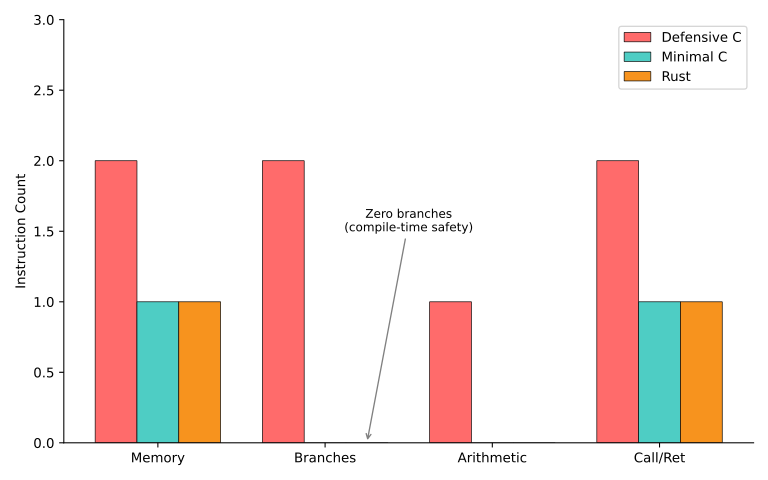
\includegraphics[width=0.48\colwidth]{../paper/figures/instruction_breakdown.pdf}
			\end{tabular}
		\end{figure}

		\heading{Key Observations}
		\begin{itemize}
			\item \textbf{Rust matches Minimal C exactly}: 2 instructions, 0 branches
			\item \textbf{Defensive C has 3.5$\times$ overhead}: Extra instructions for state validation
			\item \textbf{Critical}: Rust has \textbf{zero conditional branches}---the compiler \textit{proved} they were unnecessary
		\end{itemize}
	\end{block}

	\begin{block}{Conclusion}
		\large
		\heading{Main Result}

		Rust's typestate pattern achieves \textbf{zero-cost safety}: compile-time type checking eliminates runtime overhead while preventing invalid state transitions.

		\heading{Implications}
		\begin{enumerate}
			\item The safety-performance trade-off is \textbf{not fundamental}
			\item Sufficiently expressive type systems move verification cost to compilation
			\item This principle extends beyond memory safety to protocol correctness
		\end{enumerate}

		\heading{Broader Lesson}

		Computer science repeatedly faces ``when to pay the cost'' decisions. Understanding these trade-offs---compile vs.\ run, write vs.\ read, encode vs.\ transmit---enables better engineering choices.
	\end{block}

	\begin{block}{References}
		\footnotesize
		\begin{itemize}
			\item Microsoft Security Response Center: ``We need a safer systems programming language'' (2019)
			\item CISA: ``The urgent need for memory safety in software products'' (2024)
			\item R.\ E.\ Strom \& S.\ Yemini: ``Typestate: A programming language concept for enhancing software reliability.'' \textit{IEEE TSE}, 1986.
			\item Rust Embedded Working Group: ``Zero cost abstractions.'' \texttt{doc.rust-lang.org}
		\end{itemize}
	\end{block}

\end{column}

\separatorcolumn
\end{columns}
\end{frame}

\end{document}
